\chapter{神经网络的应用实例}
\label{cha:usecase}
\section{二维分类问题}

首先我们将刚构建的神经网络应用到二维分类问题上,第一个解决的问题是圆形分类问题,即划定一个圆,检测某个点是否在圆内。所以构建的神经网络需要接收两个输入,一个是该点的$X$位置,一个是该点的$Y$位置。为了使得位置数值归一化,点的位置限定在了$0$到$1$之间。如图~\ref{fig:case1:traindata},为随机生成的测试数据集,红色实心点代表在半径为$0.5$,圆心为$(0.5,0.5)$的圆内的点,绿色空心点为在该圆外的点。

\begin{figure}[h] 
 \centering
  \includegraphics[scale=0.8]{case1/traindata}
  \caption{测试集数据}
  \label{fig:case1:traindata}
\end{figure}

构造数据集的代码如下:

\begin{lstlisting}
%% 构造数据集
data_len = 1000;
data = zeros(data_len,3);
data(:,1:2) = rand(data_len,2);
for i=1:data_len
    data(i,3) = ((data(i,1)-0.5)^2+(data(i,2)-0.5)^2) <= 0.25^2;
end

gindex = find(data(:,3)==0);
rindex = find(data(:,3)==1);

figure;
scatter(data(rindex,1),data(rindex,2),'filled','r');
hold on;
scatter(data(gindex,1),data(gindex,2),'g');
title('训练集数据');
\end{lstlisting}

训练的网络结构使用三层神经元结构,输入层有两个神经元,隐含层有七个神经元,输出层有一个神经元。设置学习步长$step$为$0.5$,期望最高错误率为$1$\%。训练过程的代码如下:

\begin{lstlisting}
%% 训练
levels = [2,7,1];

[W,theta,record] = BP_tranning(data,levels,0.5,3,@compute_error);
\end{lstlisting}

其中$compute\_error$函数如下:

\begin{lstlisting}
function [ error ] = compute_error(output,target)
%COMPUTE_ERROR 此处显示有关此函数的摘要
%   此处显示详细说明
    output(output>0.5)=1;
    output(output<=0.5)=0;
    delta = abs(output - target);
    error = sum(sum(delta))/size(delta,2)*100;
end
\end{lstlisting}

测试神经网络准确性的代码如下:

\begin{lstlisting}
%% 测试
data_len = 1000;
data = zeros(data_len,3);
data(:,1:2) = rand(data_len,2);
for i=1:data_len
    data(i,3) = ((data(i,1)-0.5)^2+(data(i,2)-0.5)^2) <= 0.25^2;
end

Y = predict(data(:,1:2),W,theta);

Y(Y>0.5)=1;
Y(Y<=0.5)=0;
T = data(:,3) - Y';
correct_index = find(T == 0);
green_index = find(data(:,3)==0);
error_index = find(T ~= 0);
red_index = find(data(:,3)==1);

figure;
scatter(data(green_index,1),data(green_index,2),'g');
hold on
scatter(data(red_index,1),data(red_index,2),'filled','r');
title('分类测试结果')
figure;
scatter(data(correct_index,1),data(correct_index,2),'g');
hold on
scatter(data(error_index,1),data(error_index,2),'filled','r');
title('正确点和错误点')
figure;
plot(record);
title('历史错误率');
xlabel('次数');
ylabel('错误率');
\end{lstlisting}

经过分类测试的结果如图~\ref{fig:case1:result}。正确点和错误点图为图~\ref{fig:case1:incorrect},其中,红色实心点代表错误点,绿色空心点代表正确点。历史错误率如图~\ref{fig:case1:record}。

\begin{figure}[h] 
 \centering
  \includegraphics[scale=0.8]{case1/result}
  \caption{分类测试结果}
  \label{fig:case1:result}
\end{figure}
\begin{figure}[h] 
 \centering
  \includegraphics[scale=0.8]{case1/incorrect}
  \caption{正确点和错误点}
  \label{fig:case1:incorrect}
\end{figure}
\begin{figure}[h] 
 \centering
  \includegraphics[scale=0.8]{case1/record}
  \caption{历史错误率}
  \label{fig:case1:record}
\end{figure}

现将这个神经网络模型运用到双曲线分类问题中,随机生成的数据集如图~\ref{fig:case2:traindata}

\begin{figure}[h] 
 \centering
  \includegraphics[scale=0.8]{case2/traindata}
  \caption{测试集数据}
  \label{fig:case2:traindata}
\end{figure}

构造数据集的代码如下:

\begin{lstlisting}
%% 构造数据集
data_len = 1000;
data = zeros(data_len,3);
data(:,1:2) = rand(data_len,2);
for i=1:data_len
    data(i,3) = ((data(i,1)-0.5)^2-(data(i,2)-0.5)^2) <= 0.25^2;
end

gindex = find(data(:,3)==0);
rindex = find(data(:,3)==1);

figure;
scatter(data(rindex,1),data(rindex,2),'filled','r');
hold on;
scatter(data(gindex,1),data(gindex,2),'g');
title('训练集数据');
\end{lstlisting}

训练的网络结构使用三层神经元结构,输入层有两个神经元,隐含层有七个神经元,输出层有一个神经元。设置学习步长$step$为$0.5$,期望最高错误率为$1$\%。训练过程的代码如下:

\begin{lstlisting}
%% 训练
levels = [2,7,1];

[W,theta,record] = BP_tranning(data,levels,0.5,3,@compute_error);
\end{lstlisting}

其中$compute\_error$函数如下:

\begin{lstlisting}
function [ error ] = compute_error(output,target)
%COMPUTE_ERROR 此处显示有关此函数的摘要
%   此处显示详细说明
    output(output>0.5)=1;
    output(output<=0.5)=0;
    delta = abs(output - target);
    error = sum(sum(delta))/size(delta,2)*100;
end
\end{lstlisting}

测试神经网络准确性的代码如下:

\begin{lstlisting}
%% 测试
data_len = 1000;
data = zeros(data_len,3);
data(:,1:2) = rand(data_len,2);
for i=1:data_len
    data(i,3) = ((data(i,1)-0.5)^2-(data(i,2)-0.5)^2) <= 0.25^2;
end

Y = predict(data(:,1:2),W,theta);

Y(Y>0.5)=1;
Y(Y<=0.5)=0;
T = data(:,3) - Y';
correct_index = find(T == 0);
green_index = find(data(:,3)==0);
error_index = find(T ~= 0);
red_index = find(data(:,3)==1);

figure;
scatter(data(green_index,1),data(green_index,2),'g');
hold on
scatter(data(red_index,1),data(red_index,2),'filled','r');
title('分类测试结果')
figure;
scatter(data(correct_index,1),data(correct_index,2),'g');
hold on
scatter(data(error_index,1),data(error_index,2),'filled','r');
title('正确点和错误点')
figure;
plot(record);
title('历史错误率');
xlabel('次数');
ylabel('错误率');
\end{lstlisting}

经过分类测试的结果如图~\ref{fig:case2:result}。正确点和错误点图为图~\ref{fig:case2:incorrect},其中,红色实心点代表错误点,绿色空心点代表正确点。历史错误率如图~\ref{fig:case2:record}。

\begin{figure}[h] 
 \centering
  \includegraphics[scale=0.8]{case2/result}
  \caption{分类测试结果}
  \label{fig:case2:result}
\end{figure}
\begin{figure}[h] 
 \centering
  \includegraphics[scale=0.8]{case2/incorrect}
  \caption{正确点和错误点}
  \label{fig:case2:incorrect}
\end{figure}
\begin{figure}[h] 
 \centering
  \includegraphics[scale=0.8]{case2/record}
  \caption{历史错误率}
  \label{fig:case2:record}
\end{figure}

\section{三维分类问题}

现将这个神经网络模型运用到三维球形分类问题中,随机生成的数据集如图~\ref{fig:case3:traindata}

\begin{figure}[h] 
 \centering
  \includegraphics[scale=0.8]{case3/traindata}
  \caption{测试集数据}
  \label{fig:case3:traindata}
\end{figure}

构造数据集的代码如下:

\begin{lstlisting}
%% 构造数据集
data_len = 1000;
data = zeros(data_len,4);
data(:,1:3) = rand(data_len,3);
for i=1:data_len
    data(i,4) = ((data(i,1)-0.5)^2+(data(i,2)-0.5)^2+(data(i,3)-0.5)^2) <= 0.25^2;
end

gindex = find(data(:,4)==0);
rindex = find(data(:,4)==1);

figure;
scatter3(data(rindex,1),data(rindex,2),data(rindex,3),'filled','r');
hold on;
scatter3(data(gindex,1),data(gindex,2),data(gindex,3),'g');
title('训练集数据');
\end{lstlisting}

训练的网络结构使用三层神经元结构,输入层有三个神经元,隐含层有七个神经元,输出层有一个神经元。设置学习步长$step$为$0.5$,期望最高错误率为$1$\%。训练过程的代码如下:

\begin{lstlisting}
%% 训练
levels = [3,7,1];

[W,theta,record] = BP_tranning(data,levels,0.5,1,@compute_error);
\end{lstlisting}

其中$compute\_error$函数如下:

\begin{lstlisting}
function [ error ] = compute_error(output,target)
%COMPUTE_ERROR 此处显示有关此函数的摘要
%   此处显示详细说明
    output(output>0.5)=1;
    output(output<=0.5)=0;
    delta = abs(output - target);
    error = sum(sum(delta))/size(delta,2)*100;
end
\end{lstlisting}

测试神经网络准确性的代码如下:

\begin{lstlisting}
%% 测试
data_len = 1000;
data = zeros(data_len,4);
data(:,1:3) = rand(data_len,3);
for i=1:data_len
    data(i,4) = ((data(i,1)-0.5)^2+(data(i,2)-0.5)^2+(data(i,3)-0.5)^2) <= 0.25^2;
end

Y = predict(data(:,1:3),W,theta);

Y(Y>0.5)=1;
Y(Y<=0.5)=0;
T = data(:,4) - Y';
correct_index = find(T == 0);
green_index = find(data(:,4)==0);
error_index = find(T ~= 0);
red_index = find(data(:,4)==1);

figure;
scatter3(data(green_index,1),data(green_index,2),data(green_index,3),'g');
hold on
scatter3(data(red_index,1),data(red_index,2),data(red_index,3),'filled','r');
title('分类测试结果')
figure;
scatter3(data(correct_index,1),data(correct_index,2),data(correct_index,3),'g');
hold on
scatter3(data(error_index,1),data(error_index,2),data(error_index,3),'filled','r');
title('正确点和错误点')
figure;
plot(record);
title('历史错误率');
xlabel('次数');
ylabel('错误率');
\end{lstlisting}

经过分类测试的结果如图~\ref{fig:case3:result}。正确点和错误点图为图~\ref{fig:case3:incorrect},其中,红色实心点代表错误点,绿色空心点代表正确点。历史错误率如图~\ref{fig:case3:record}。

\begin{figure}[h] 
 \centering
  \includegraphics[scale=0.8]{case3/result}
  \caption{分类测试结果}
  \label{fig:case3:result}
\end{figure}
\begin{figure}[h] 
 \centering
  \includegraphics[scale=0.8]{case3/incorrect}
  \caption{正确点和错误点}
  \label{fig:case3:incorrect}
\end{figure}
\begin{figure}[h] 
 \centering
  \includegraphics[scale=0.8]{case3/record}
  \caption{历史错误率}
  \label{fig:case3:record}
\end{figure}